% Paper outline (Update 8): every section in bullet points. The text is written in later updates
% (Setup in Update 9, Introduction in Update 11, Related Work in Update 12, Method in Update 13,
% the rest in Update 15). Numbers come from results/; check them again before the final version.
%
% Build: from this folder, e.g. `tectonic main.tex` or `pdflatex main.tex`.
% The figures are read from ../results/figures/.
\documentclass[conference]{IEEEtran}

\usepackage[T1]{fontenc}
\usepackage{graphicx}
\usepackage{booktabs}
\usepackage{url}
\graphicspath{{../results/figures/}}

\begin{document}

\title{Silent Tool-Call Failures: How Quantization Degrades Function Calling and Structured Output in Small LLMs}

% Author list and affiliation: to be confirmed with the supervisor.
\author{\IEEEauthorblockN{Shawal Kabir Chy.}
\IEEEauthorblockA{CSE498R Directed Research\\
Supervisor: Dr.\ Mohammad Shifat-E-Rabbi}}

\maketitle

\begin{abstract}
\textit{Outline. Written last (Update 15).}
\begin{itemize}
  \item Problem: small LLMs run quantized on local devices, and a wrong tool call is a wrong action.
        Accuracy alone does not show how the calls fail.
  \item What we do: 5 models (1--8B) $\times$ 5 precisions $\times$ 2 decoding modes on the 1,390
        non-live BFCL questions, one serving stack; every failure sorted into syntactic and semantic classes;
        paired significance tests.
  \item Findings so far: Qwen3-4B and Qwen3-8B stay within 2.35 points of FP16 at every precision; the
        three smaller models move by up to 33 points, mostly through format; 11 of 20 changes are significant.
  \item Headline: constrained decoding removes a quantization loss only when it is a format error over the
        right content (68--111\% of three significant losses removed); it leaves content losses unchanged, and
        it makes two losses larger, where the model answers with no call instead.
  \item Schema stress (RQ4): no schema feature breaks across the board; the clearest case, objects nested three
        levels deep in Qwen3-4B at 4 bits, fails in format only, and the other weak spots are already there at FP16.
\end{itemize}
\end{abstract}

\section{Introduction}
% First draft (Update 11); RQ4 results added in Update 12. Citations are added as BibTeX in Update 16.
Language models that act as agents answer with function calls: a request to book a room, move money or switch a
device becomes a call with a function name and typed arguments, which a program then executes. On laptops, phones
and on-premise servers these agents usually run small models, and usually in a quantized form, most often with
4-bit weights. Quantization is mostly judged by perplexity or chat benchmarks, but a function call is stricter
than chat: it must be valid JSON, match the function's schema, and carry the right values. When quantization
breaks a call, the failure is often silent. The reply may not parse, so the action is dropped, or it may parse
and fit the schema while an argument is wrong, so the wrong action is taken.

Earlier work has measured tool use under quantization. ACBench reports aggregate tool-use scores for GPTQ and
AWQ models from 2B to 32B parameters and finds only small drops at 4 bits. Less is More reports large drops for a
quantized Llama-3.1-8B on BFCL questions, but its full-precision and quantized models run on different serving
stacks. Jang et al.\ count failures per channel for 9B to 35B models in multi-turn tasks, and Wu et al.\ study
which tool-use decisions flip at 2 to 4 bits. Constrained decoding, which forces a reply to match a JSON schema,
has been studied at full precision. What these studies leave open is how the function calls of small models fail
at the common precisions when everything else is held fixed, and whether constrained decoding removes the damage
that quantization does.

We therefore run five instruction-tuned models from two families (Qwen3-1.7B, 4B and 8B, and Llama-3.2-1B and
3B) at five precisions (FP16, INT8, NF4, GPTQ and AWQ) and in two decoding modes (free and
JSON-schema-constrained) on the 1,390 non-live questions of the Berkeley Function Calling Leaderboard (BFCL), all with one
serving stack (vLLM) on one kind of GPU. We ask four research questions:
\begin{enumerate}
  \item[\textbf{RQ1}] How much does function-calling accuracy change at each precision, and does the change depend
        on model size?
  \item[\textbf{RQ2}] How much of each change is syntactic (the reply is not valid JSON or does not match the
        schema), and how much is semantic (a well-formed call that is wrong)?
  \item[\textbf{RQ3}] How much of the quantization penalty does constrained decoding remove, and which failures
        remain?
  \item[\textbf{RQ4}] Which schema features (nested objects, enumerated values, integer and float arguments,
        optional arguments, non-ASCII strings and large tool menus) break first as precision drops?
\end{enumerate}

The two larger Qwen3 models stay within 2.35 points of FP16 at every precision, while the three smaller models
move by up to 33 points, mostly through format; 11 of the 20 changes are statistically significant. Constrained
decoding removes a quantization loss only when the loss is a format error over the right content: it removes
68--111\% of three significant losses, leaves the losses of the two larger models unchanged, and makes two losses
larger, because the forced model answers with no call instead. On a schema-stress suite of 175 questions, no schema
feature breaks across the board as precision drops: the clearest case, objects nested three levels deep in Qwen3-4B
at 4 bits, fails in format only, and the other weak spots are already there at FP16.

Our contributions are:
\begin{itemize}
  \item a controlled sweep of 50 runs (5 models $\times$ 5 precisions $\times$ 2 decoding modes) with pinned model
        revisions, greedy decoding and one serving stack;
  \item a classifier that sorts every failed call into two syntactic and five semantic classes, checked by hand on
        80 failures;
  \item paired significance tests for every change, so that real changes can be told from chance;
  \item a comparison of free and constrained decoding that shows which quantization losses a schema can remove;
  \item a schema-stress suite of 175 questions in seven groups, one per schema feature plus a control;
  \item code, configurations, raw answers and scores, released for reproduction.
\end{itemize}
We do not claim to be the first to evaluate quantized models on tool calling (Section~\ref{sec:related}).

\section{Related Work}\label{sec:related}
% First draft (Update 12), from notes/related_work.md; literature checked again on 10 Nov 2026.
\textbf{Quantization and tool calling.} ACBench evaluates compressed models from 2B to 32B parameters, GPTQ and AWQ
among them, on agent tasks that include tool use, and finds that 4-bit weights cost only 1--3\% on tool use; it
reports aggregate scores. Less is More shows Llama-3.1-8B falling from 63\% to 20--44\% on 230 BFCL questions in 4-
to 8-bit builds, but its full-precision model and its quantized builds run on different serving stacks. TinyAgent
keeps the success rate of fine-tuned 1.1B and 7B agents at 4 bits, after quantization-aware fine-tuning on one task.
Recent preprints look closer. Jang et al.\ find that the task score of 9B to 35B models stays flat while tool-name
hallucinations grow up to 2.5 times, and that malformed arguments stay near zero. Wu et al.\ find that at low bit
widths the decision whether to call a tool flips before the choice of tool, while argument filling barely flips.
Hu shows that the comparison of 8-bit and 4-bit models recovering from tool failures can change direction with the
prompt and the scoring rule, which argues for matched questions and a stated scoring policy. The open-source
QuantCliff project runs GGUF builds of three models with and without a JSON-schema grammar and finds that the grammar
removes malformed output without raising task success. AgentQ shows, as an attack, that a model can be built to make
harmful function calls only after it is quantized to NF4, FP4 or INT8.

\textbf{Quantization beyond perplexity.} Studies of quantized code models find that quantization methods differ
widely (Afrin et al.), and on-device evaluations report accuracy, latency and memory. Neither checks whether
structured output stays valid.

\textbf{Function-calling evaluation.} BFCL is the standard benchmark: it checks each call against possible answers
and compares models, not the precisions of one model. ToolScan sorts the errors of tool-using models into a
taxonomy, at full precision. Our failure classes follow the same idea, but they are tied to the schema that
constrained decoding enforces, so the syntactic share is exactly what a schema can block.

\textbf{Structured output and constrained decoding.} At full precision, format restrictions can lower reasoning
accuracy (Let Me Speak Freely?), and JSONSchemaBench compares constrained-decoding engines on 10,000 real-world
schemas. Several 2026 preprints find that a schema repairs format more than it improves content: hard schema
decoding makes every output valid but lowers the accuracy of 0.5B to 1.7B models (Ray); constraining tool names in
0.6B to 4B routers mostly repairs unreadable output (Lee); and constrained decoding removes every structural failure
of 0.6B to 4B models but leaves a semantic gap (Chavan). Li et al.\ report that some models stop calling tools when
a JSON-schema constraint and tool calling are switched on together. We use XGrammar, the backend of vLLM's guided
decoding.

\textbf{This work.} We build on these studies with a controlled sweep of small models: one prompt, scorer and serving
stack for five precisions, every failure sorted into syntactic and semantic classes, paired tests for every change,
and a test of constrained decoding against quantization on the full non-live BFCL set, which QuantCliff studied on
20 scenarios. The schema-stress suite adds a view by schema feature; JSONSchemaBench catalogues such features, but
uses them to compare decoding engines.

\section{Experimental Setup}\label{sec:setup}
% Written in Update 9. Every value below is in configs/, src/ or results/meta/.

\subsection{Models}
We study five instruction-tuned models from two families: Qwen3-1.7B, Qwen3-4B and Qwen3-8B, and
Llama-3.2-1B-Instruct and Llama-3.2-3B-Instruct. Each model is pinned to one Hugging Face revision.
Qwen3 runs with its thinking mode switched off, so that every model answers directly. Llama's chat
template writes the current date into the system prompt, so we fix that date, and every run sees the
same prompt.

\subsection{Precisions}
Each model runs at five precisions (Table~\ref{tab:precisions}). FP16 is the baseline, because the
T4 GPU does not support BF16. INT8 uses bitsandbytes 8-bit weights (outlier threshold 6.0); vLLM
loads such models only when they are already quantized, so we save the checkpoint first. NF4 uses
bitsandbytes 4-bit NormalFloat, which vLLM applies while loading the FP16 weights. GPTQ and AWQ
use 4-bit weights in groups of 128, made with GPTQModel 5.7.0: GPTQ is symmetric without activation
reordering, and AWQ uses zero points and the GEMM format. Both methods use the same calibration
data for every model: the first 256 documents of at least 3,000 characters from one file of
C4 (English), each cut to 512 tokens. Qwen3-8B AWQ needed three further settings, all about memory
or numerical overflow on the T4; its quantization settings and calibration data are unchanged.

\begin{table}[t]
\centering
\caption{The five precisions}\label{tab:precisions}
\begin{tabular}{lll}
\toprule
Precision & Weights & Made by \\
\midrule
FP16 & 16-bit & --- \\
INT8 & 8-bit, per row & bitsandbytes, saved first \\
NF4  & 4-bit, blocks of 64 & bitsandbytes, while loading \\
GPTQ & 4-bit, groups of 128 & GPTQModel \\
AWQ  & 4-bit, groups of 128 & GPTQModel \\
\bottomrule
\end{tabular}
\end{table}

\subsection{Benchmark and scoring}
We use the 1,390 non-live questions of the Berkeley Function Calling Leaderboard (BFCL, bfcl-eval
2026.3.23): 1,150 AST questions (simple in Python, Java and JavaScript; multiple; parallel;
parallel-multiple) and 240 irrelevance questions, where no function fits and the right answer is
no call. Our own runner gives the model the functions and asks for a JSON array of calls, using
BFCL's default prompt wording with only the output format changed. The parser accepts only that
array, with surrounding whitespace and at most one Markdown code fence; it repairs nothing, so a
malformed answer counts as a failure. Parsed answers are scored with BFCL's own AST checker. We
report BFCL's Non-Live Overall accuracy (the unweighted mean of simple, multiple, parallel and
parallel-multiple, where simple is the mean of its three languages) and irrelevance accuracy on its
own. On Qwen3-4B-Instruct-2507, BFCL's own harness reproduced the leaderboard on our hardware, and
our runner scored within 1.5 points of BFCL's function-calling mode.

\subsection{Inference}
All runs use vLLM 0.8.5 on NVIDIA T4 GPUs (16\,GB) on Kaggle: one GPU per run, except FP16
Qwen3-8B, which is split across two. Decoding is greedy (temperature 0, seed 42), with at most
4,096 answer tokens, the same budget as BFCL. In constrained mode, vLLM's guided decoding with the
XGrammar backend forces every answer to match a JSON schema built from the question's functions:
an array of calls, each naming one of the given functions, with its arguments typed as declared
and no extra arguments. The prompt is the same in both modes, so the constraint is the only
difference.

\section{Method}\label{sec:method}
\textit{Drafted in Update 13.}
\begin{itemize}
  \item Failure classes: S1 not valid JSON, S2 does not match the schema (syntactic); M1 wrong function,
        M2 wrong argument value, M3 wrong number of calls, M4 call on an irrelevance question, M5 no call
        (semantic). Checked in this order; the schema is the one constrained decoding enforces.
  \item Hand check: two random samples of 40 failures; the final classifier agrees on all 80.
  \item Statistics: McNemar's exact test on the 1,150 AST questions, paired by question, with Holm's
        correction over the 20 comparisons; bootstrap 95\% intervals for the change in Overall
        (10,000 resamples inside each category).
  \item Constrained-decoding gap: the penalty (change from FP16 of the same model and mode) in free and in
        constrained mode; their difference with a bootstrap 95\% interval (the same resampled questions for all
        four runs); and, for the significant free losses, the share of the loss removed.
  \item Schema-stress suite: made from templates with fixed seeds by \texttt{src/stress\_suite.py}; each question
        has one correct call, with every value stated in the question; the answer keys are checked to accept
        the correct call and reject 220 wrong ones; scored with BFCL's checker, like the main questions.
  \item Stress-suite analysis: accuracy per group and level; the failure classes above, plus whether a wrong value
        is in the stressed argument and whether an invalid answer is right once only its closing brackets are fixed;
        McNemar's exact test per group against FP16 of the same model and mode, with Holm's correction over the 140
        tests of each mode.
\end{itemize}

\section{Results}\label{sec:results}
\subsection{Accuracy by precision and model size (RQ1)}
\begin{itemize}
  \item Table~\ref{tab:main} and Fig.~\ref{fig:penalty}. Qwen3-4B and Qwen3-8B stay within 2.35 points of
        FP16; only two of their eight changes are significant.
  \item The smaller models move a lot: Qwen3-1.7B GPTQ $-33.31$; Llama-3.2-1B $-18.59$ to $-25.00$ with NF4,
        GPTQ and AWQ; Llama-3.2-3B $+8.35$ to $+28.14$ with the same three.
  \item Within each family the smallest model is hurt most. Across families, size alone does not predict the
        change: Llama-3.2-3B gains, while Qwen3-4B, of similar size, barely moves.
\end{itemize}

\begin{table}[t]
\centering
\caption{Overall accuracy (\%), free decoding}\label{tab:main}
\begin{tabular}{lrrrrr}
\toprule
Model & FP16 & INT8 & NF4 & GPTQ & AWQ \\
\midrule
Qwen3-1.7B   & 72.56 & 69.42 & 69.06 & 39.25 & 75.94 \\
Qwen3-4B     & 88.04 & 88.29 & 85.69 & 86.60 & 86.98 \\
Qwen3-8B     & 88.29 & 87.27 & 88.00 & 85.98 & 88.42 \\
Llama-3.2-1B & 36.40 & 34.94 & 16.02 & 11.40 & 17.81 \\
Llama-3.2-3B & 31.38 & 34.02 & 52.75 & 59.52 & 39.73 \\
\bottomrule
\end{tabular}
\end{table}

\begin{figure}[t]
\centering
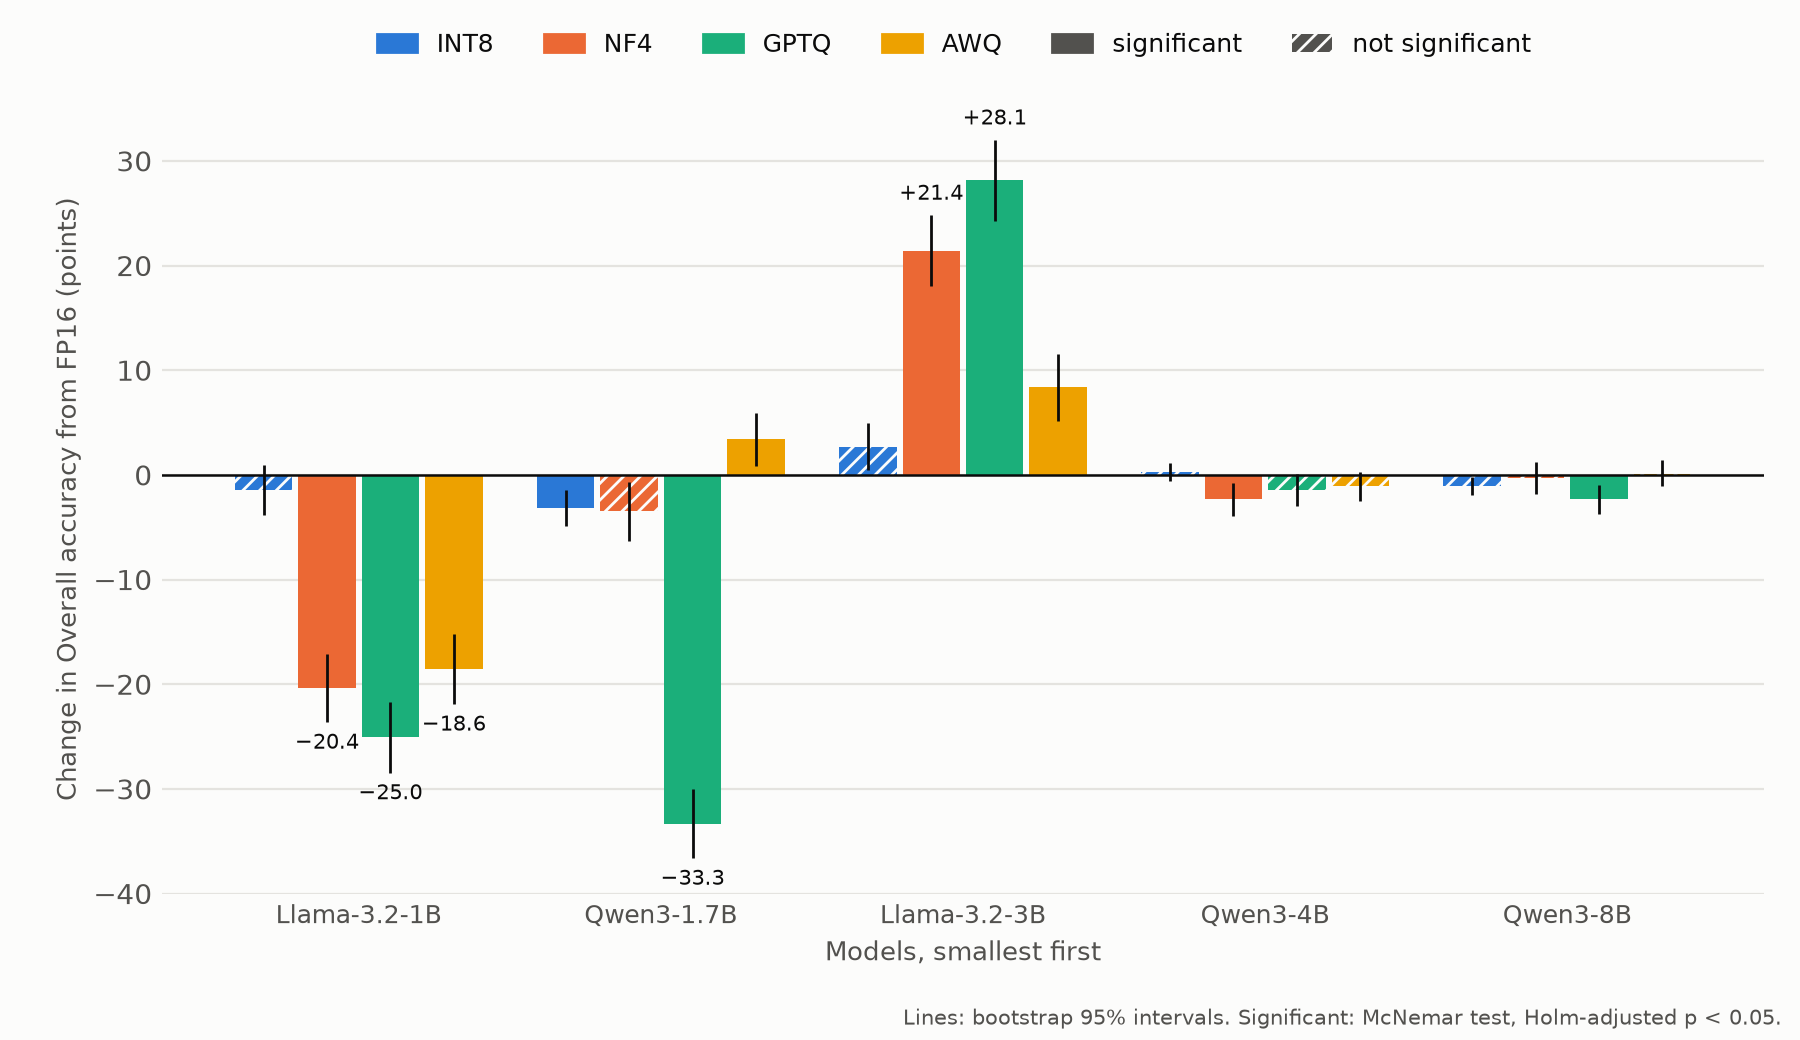
\includegraphics[width=\columnwidth]{penalty_by_size_free.png}
\caption{Change in Overall accuracy from FP16, models smallest first, with bootstrap 95\% intervals.
Striped bars are not significant (McNemar, Holm-adjusted $p \geq 0.05$).}\label{fig:penalty}
\end{figure}

\subsection{Failure classes (RQ2)}
\begin{itemize}
  \item Fig.~\ref{fig:taxonomy}. 6,844 of the 11,625 failures in the 25 free runs (58.9\%) are syntactic.
  \item Qwen3-4B and Qwen3-8B fail mostly on argument values (M2); in the smaller models, quantization mostly
        moves the syntactic counts (Qwen3-1.7B GPTQ: $+273$ syntactic, $+63$ semantic).
  \item Examples: an extra \texttt{\}} (Qwen3-1.7B GPTQ), a copied function definition (Llama-3.2-1B), a
        missing closing \texttt{]} (Llama-3.2-3B FP16).
  \item Caveat: a format error hides any content error in the same answer.
\end{itemize}

\begin{figure}[t]
\centering
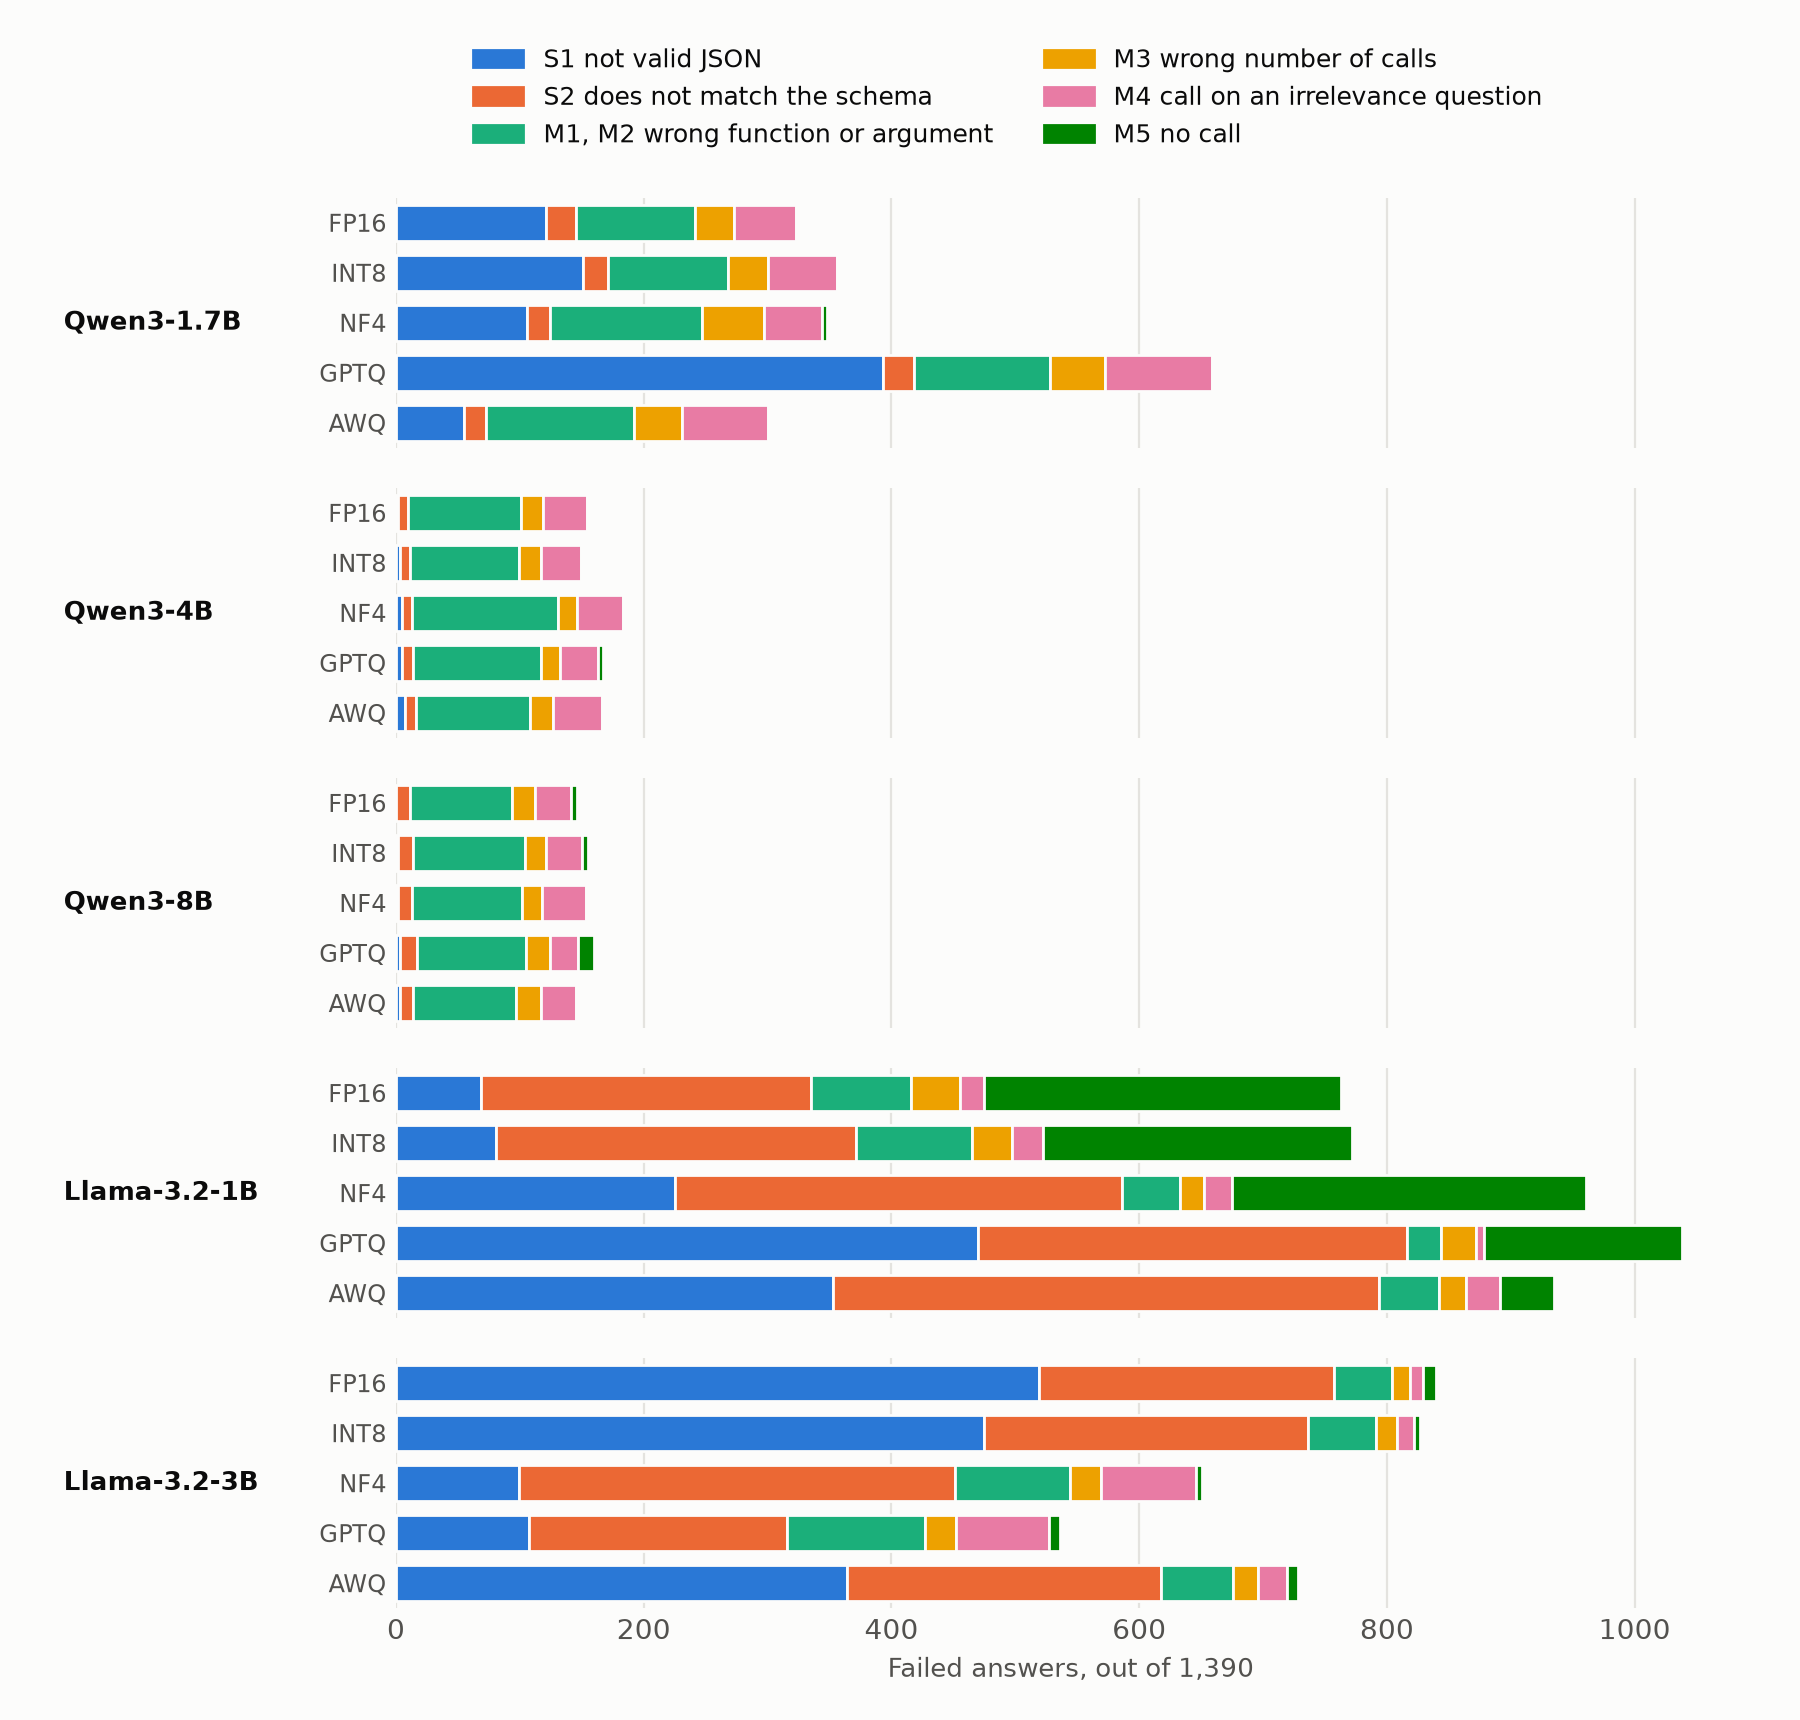
\includegraphics[width=\columnwidth]{taxonomy_free.png}
\caption{Failure classes per run, free decoding (out of 1,390 answers).}\label{fig:taxonomy}
\end{figure}

\subsection{Constrained decoding (RQ3)}
\begin{itemize}
  \item Fig.~\ref{fig:gap}. The constraint raises FP16 for every model (Llama-3.2-3B by 39.66 points) and
        24 of the 25 runs; syntactic failures fall from 6,844 to 53 (none breaks the schema).
  \item Of the 7 significant free losses: removed for Qwen3-1.7B INT8 (111\%) and GPTQ (68\%) and
        Llama-3.2-1B AWQ (98\%); unchanged for Qwen3-4B NF4 and Qwen3-8B GPTQ (content losses); larger for
        Llama-3.2-1B NF4 ($-20.38 \to -30.36$) and GPTQ ($-25.00 \to -45.29$), which answer with an empty
        array instead.
  \item Free-mode gains were format effects: Llama-3.2-3B's $+8.35$ to $+28.14$ become changes below FP16.
  \item Substitution: semantic failures rise from 4,781 to 8,902; what is left is wrong values (Qwen3), no call
        (Llama-3.2-1B), and a mix (Llama-3.2-3B). Under the constraint, 8 of the 20 changes are significant.
\end{itemize}

\begin{figure}[t]
\centering
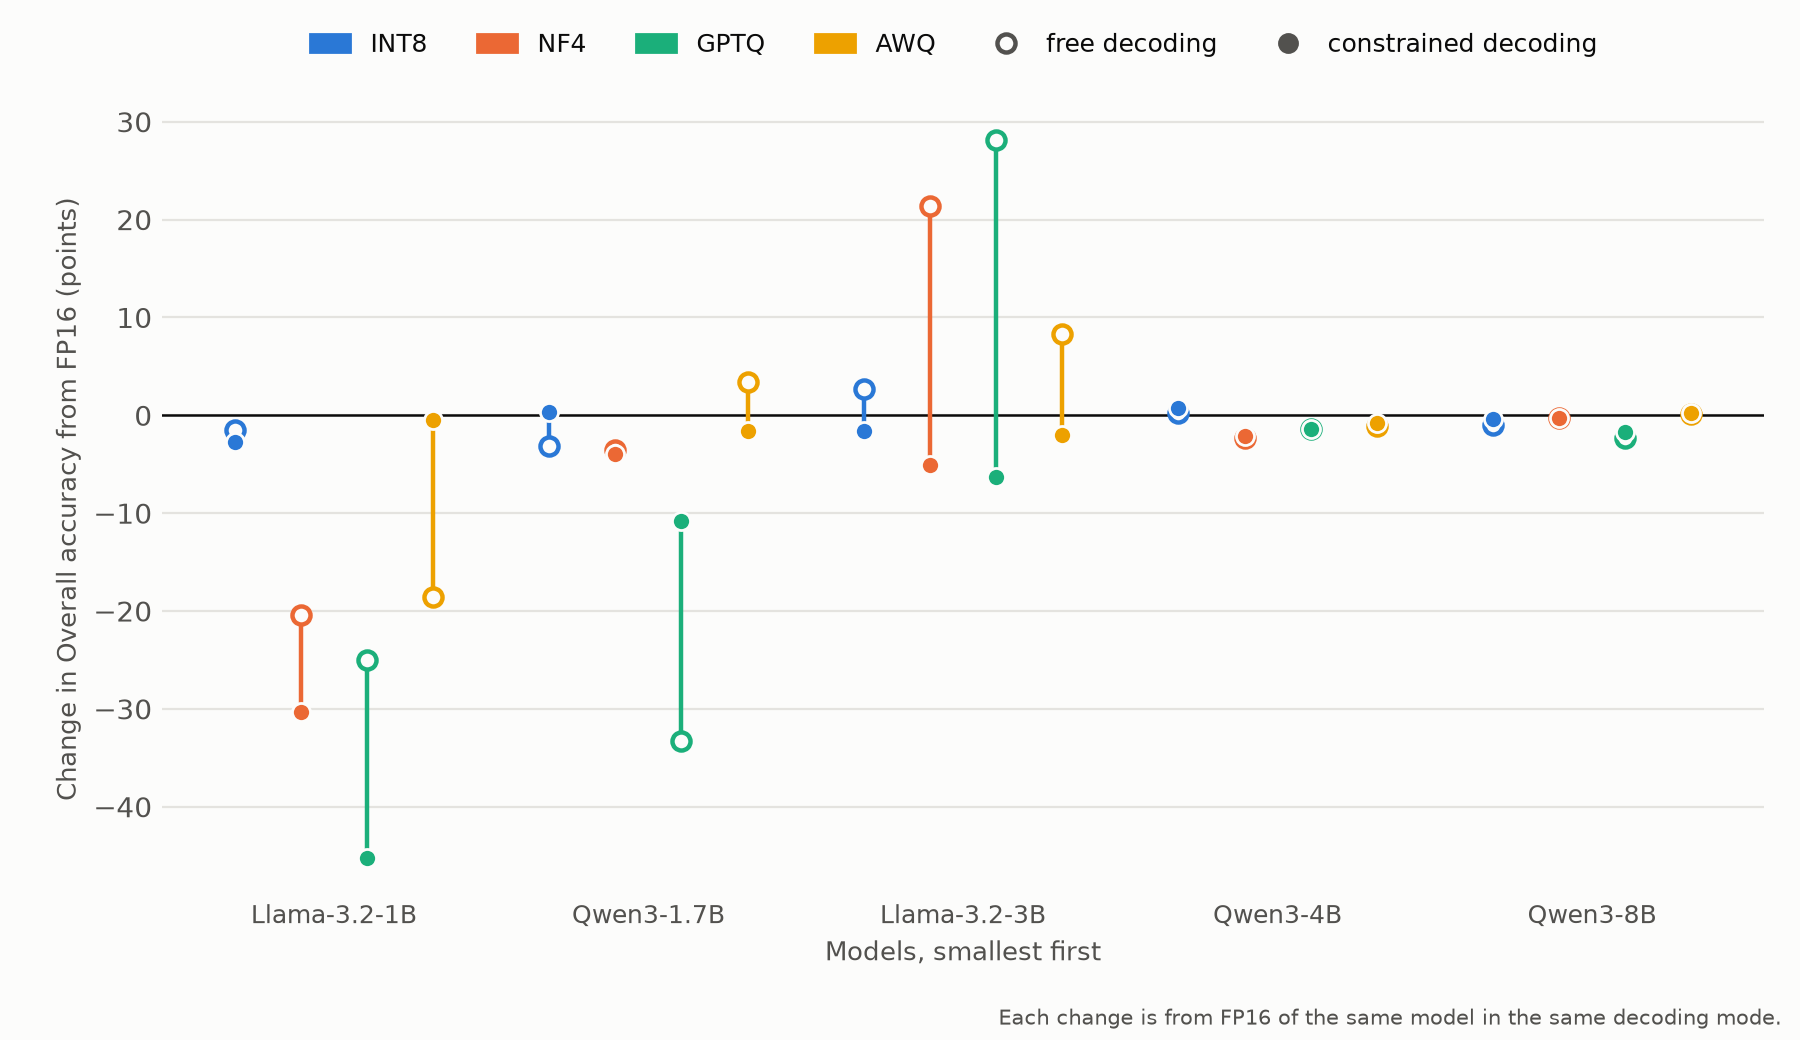
\includegraphics[width=\columnwidth]{constrained_gap.png}
\caption{Change in Overall accuracy from FP16 with free decoding (open circles) and constrained decoding
(filled circles), models smallest first.}\label{fig:gap}
\end{figure}

\subsection{Schema-stress suite (RQ4)}
\begin{itemize}
  \item Table~\ref{tab:stress}. 175 questions in seven groups of 25 (nested objects, enumerated codes, integer and
        float arguments, optional arguments, non-ASCII strings, 50-function menus, and a plain control), 50 runs.
  \item No feature breaks across the board. Qwen3-4B and Qwen3-8B miss at most 2 questions in any constrained run.
  \item The clearest case is three-level nesting in Qwen3-4B with free decoding: 6 of 6 right at FP16, 5 at INT8,
        none at NF4, GPTQ and AWQ. All 19 failures are wrong closing braces over the right content (each is right
        once only the brackets are fixed); with the constraint every precision gets 6 of 6. The drop is the same for
        all three 4-bit methods but does not pass Holm's correction: a group of 25 must lose 13 to pass.
  \item The other weak spots are there at FP16: Qwen3-1.7B adds a closing brace after a number (44 of its 125 number
        answers in free decoding, FP16 the worst), Llama-3.2-3B miswrites non-ASCII letters as \texttt{\textbackslash u}
        escapes (5--8 of 25 with the constraint), and Llama-3.2-1B answers 23 of the 25 control questions at FP16
        with no call.
  \item No well-formed answer has a wrong number: the 104 wrong values in the number group are all in an ID
        argument. In the enum, optional and unicode groups every wrong value is in the stressed argument; with 30
        codes, Qwen3-1.7B GPTQ picks a wrong code on 4 of 8 questions.
  \item 7 of the 280 changes pass Holm's correction: three gains in free decoding (two in format, one in fewer empty
        answers), and, under the constraint, Llama-3.2-1B's empty answers and its gains on the menu.
\end{itemize}

\begin{table*}[t]
\centering
\caption{Schema-stress suite: correct answers out of 25 per group at FP16, with the lowest and highest of the four
quantized precisions in brackets}\label{tab:stress}
\begin{tabular}{llrrrrrrr}
\toprule
Mode & Model & Plain & Nested & Enum & Number & Optional & Unicode & Menu \\
\midrule
Free & Qwen3-1.7B & 25 (25) & 24 (20--25) & 22 (21--23) & 9 (13--25) & 25 (23--25) & 24 (23--24) & 25 (22--25) \\
 & Qwen3-4B & 25 (25) & 25 (19--24) & 25 (24--25) & 25 (25) & 25 (25) & 25 (24--25) & 25 (24--25) \\
 & Qwen3-8B & 25 (25) & 25 (25) & 25 (24--25) & 25 (25) & 25 (25) & 25 (25) & 25 (25) \\
 & Llama-3.2-1B & 2 (2--16) & 11 (0--18) & 5 (0--3) & 3 (0--11) & 14 (8--20) & 4 (1--7) & 3 (0--3) \\
 & Llama-3.2-3B & 16 (16--25) & 12 (14--24) & 11 (8--23) & 9 (5--11) & 7 (9--23) & 5 (1--7) & 19 (18--25) \\
\midrule
Constrained & Qwen3-1.7B & 25 (25) & 25 (25) & 22 (21--23) & 25 (25) & 25 (25) & 24 (23--24) & 25 (23--25) \\
 & Qwen3-4B & 25 (25) & 25 (25) & 25 (24--25) & 25 (25) & 25 (25) & 25 (24--25) & 25 (25) \\
 & Qwen3-8B & 25 (25) & 25 (25) & 25 (24--25) & 25 (25) & 25 (25) & 25 (25) & 25 (25) \\
 & Llama-3.2-1B & 2 (0--4) & 20 (0--23) & 8 (0--9) & 9 (0--7) & 12 (1--9) & 6 (0--7) & 6 (3--25) \\
 & Llama-3.2-3B & 25 (21--25) & 25 (21--25) & 24 (20--25) & 13 (12--15) & 25 (25) & 8 (5--8) & 22 (10--24) \\
\bottomrule
\end{tabular}
\end{table*}

\subsection{Memory and speed}
\begin{itemize}
  \item Weights per GPU and output tokens per second for every run, from \texttt{results/meta/}.
\end{itemize}

\section{Discussion}
\textit{Update 15.}
\begin{itemize}
  \item For small models, format habits decide much of the score, and quantization changes those habits in
        both directions.
  \item A higher score after quantization (Llama-3.2-3B) comes mostly from better format, not better content.
  \item What this means for running agents on small quantized models.
\end{itemize}

\section{Limitations}
\begin{itemize}
  \item FP16, not BF16, as the baseline (T4 GPUs); models of 8B or smaller; two model families.
  \item One run per configuration (greedy decoding); single-turn BFCL questions only.
  \item One calibration set for GPTQ and AWQ; Qwen3-8B AWQ needed extra settings.
  \item The schema is very slightly stricter than BFCL's checker (14 of 34,750 correct answers).
  \item The stress groups are small (25 questions, 6--9 per level); the number group also has an ID argument, and
        the menu functions have no argument descriptions.
\end{itemize}

\section{Conclusion}
\textit{Update 15.}
\begin{itemize}
  \item Answers to RQ1--RQ4 in one paragraph each; the practical advice.
\end{itemize}

\section*{References}
\textit{To be added as BibTeX (Update 16): BFCL, ToolScan, ACBench, Less is More, TinyAgent, Jang et al.,
Wu et al., Hu, AgentQ, QuantCliff, Afrin et al., the on-device evaluation, the constrained-decoding papers
(Let Me Speak Freely?, JSONSchemaBench, Ray, Li et al., Lee, Chavan), vLLM, XGrammar, GPTQ, AWQ, LLM.int8(), QLoRA.}

\end{document}
